\section{Evaluierung und Optimierung} \label{eval}

% http://stats.stackexchange.com/questions/118219/how-to-interpret-matthews-correlation-coefficient-mcc

In diesem Kapitel untersuchen wir, welchen Einfluss unterschiedliche Features und Verfahren auf die Qualität eines binären Klassifikators haben.

% TODO eigentlich gehen wir auf die Experimente ein
Dabei gehen wir zunächst auf das generelle Vorgehen bei den Experimenten ein und betrachten anschließend einige der in Kapitel \ref{Features} besprochenen Features näher. Danach führen wir verschiedene Methoden zur Bewertung von Klassifikatoren ein und untersuchen anhand dieser die in Kapitel \ref{Klassifikatoren} angesprochenen Klassifikatoren.
Schließlich untersuchen wir auch die Laufzeit der unterschiedlichen Verfahren.


\subsection{Vorgehen}

%TODO eigentlich verwendet man 10-fache stratifizierte Kreuzvalidierung

Als Grundlage der in diesem Kapitel besprochenen Untersuchungen dienen die in Kapitel \ref{DataSimulation} betrachteten Datensätze, also simulierte Quader, Zylinder und zwei Arten von Kugeln. Bei jedem Experiment werden zwei dieser Datensätze verwendet und zwischen den entsprechenden Teilchenarten unterschieden. Dabei werden die Datensätze zunächst gelabelt, kombiniert und in eine zufällige Reihenfolge gebracht. Anschließend wird mit Hilfe dieser Daten ein Klassifikator über eine 10-fache Kreuzvalidierung trainiert und bestimmte Parameter, z. B. der F1-Score, evaluiert. Dieser Vorgang wird für jeden Parameter mehrmals (TODO wie oft) wiederholt und der Mittelwert als Ergebnis verwendet.

Die 10-fache Kreuzvalidierung dient dabei dazu die Varianz der Abschätzung möglichst klein zu halten und ist nach Kohavi \cite{Kohavi95astudy} in der Praxis das beste Verfahren zur Modellauswahl (TODO model selection), also zur Auswahl des besten Klassifikators aus einer gegebenen Menge von Klassifikatoren.






\subsection{Bewertungsverfahren}

(TODO: Jeweils auf den Wertebereich eingehen. Geht bei einigen von 0 bis 1 und bei anderen von -1 bis 1)

Es gibt zahlreiche Metriken mit denen sich die Qualität eines Klassifikators feststellen lässt. Einen guten Überblick geben zum Beispiel Baldi et al. \cite{Baldi2000} und Powers \cite{Powers2011}. Als Grundlage für all diese Metriken dient die sogenannte Kontingenztafel (siehe Abbildung TODO). Diese enthält insbesondere die Anzahl an True-Positives, False-Positives, True-Negatives und False-Negatives, die wir im Kontext von mathematischen Formeln mit TP, FP, TN und FN abkürzen werden.

In dieser Arbeit wird versucht einen Kompromiss zwischen besonders anschaulichen und bezüglich der Modellauswahl besonders aussagekräftigen Verfahren zu finden.

\begin{figure}[!h]
    \centering
    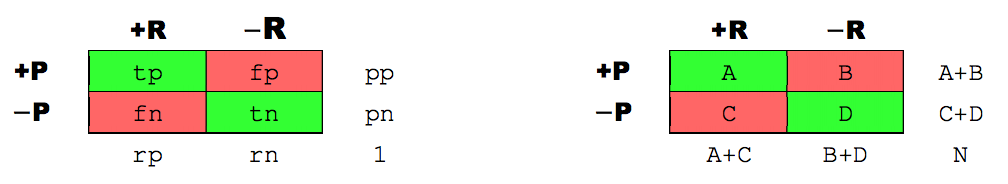
\includegraphics[width=0.7\textwidth]{pics/contingency.png}
    \caption{Kontingenztafel \cite{Powers2011}}
    \label{fig:VergleichScores}
\end{figure}


\paragraph{F1-Score}

Eines der besonders anschaulichen Verfahren ist der F1-Score. Dieser ist das harmonische Mittel zwischen Precision und Recall (siehe Formel \ref{f1Score}). Da Precision ein Maß dafür ist, wie gut der Klassifikator False-Positives vermeidet, und Recall beschreibt wie gut False-Negatives vermieden werden, beschreibt ein guter F1-Score also ein Verfahren, dass wenige Typ I und Typ II Fehler verursacht.

Allerdings sind Precision und Recall und damit der F1-Score unabhängig von der Anzahl an True-Negatives. Daher ist der F1-Score nur bedingt zur Modellauswahl geeignet. 
Ein weiteres Problem des F1-Scores ist, dass er in gewisser Weise biased ist. Man könnte beispielsweise eine reale Anwendung haben in der es wichtiger ist False Positives zu vermeiden, als False Negatives. Man kann dies umgehen, indem man die beiden Summanden im harmonischen Mittel unterschiedlich gewichtet, muss sich dafür aber auf eine Gewichtung festlegen. Diese Metriken nennt man dann F-Scores.

Dennoch wird der F1-Score, u.a. auf Grund seiner Anschaulichkeit, gerne verwendet. Man sollte ihn allerdings nicht als alleiniges Maß nutzen.

\begin{eqnarray} \label{f1Score}
    \hspace{1cm} F_1 = 2 \cdot \frac{1}{\frac{1}{PPV} + \frac{1}{TPR}} = 2 \cdot \frac{PPV \cdot TPR}{PPV + TPR} \text{\hspace{1cm}(F1-Score)}\\
    \hspace{1cm} PPV = \frac{TP}{TP + FP} \text{\hspace{1cm}(Precision / Positive Predictive Value)} \\
    \hspace{1cm} TPR = \frac{TP}{TP + FN} \text{\hspace{1cm}(Recall)}
\end{eqnarray}


\paragraph{ROC}

Wie oben erwähnt hat der F1-Score einige Probleme. Eine Möglichkeit diese zu umgehen, ist die ROC-Kurve.
Dabei trägt man in einer Grafik entlang der x-Achse die False-Positive-Rate (FPR) auf und entlang der y-Achse die True-Positive-Rate (TPR). Man verwendet dann einen Klassifikator, bei dem man frei einstellen kann, wie wichtig das Maximieren der True-Positive-Rate gegenüber dem Minimieren der False-Positive-Rate ist. Zu jeder dieser Einstellungen misst man dann jeweils die True-Positive-Rate und die False-Positive-Rate und trägt an der entsprechenden Stelle in der Grafik einen Datenpunkt ein. So ergibt sich über eine Vielzahl von Messungen eine Kurve, die man als ROC-Kurve bezeichnet (siehe z. B. Grafik TODO).

%TODO Bias definieren
Wie man schon am Vorgehen zur Bestimmung der ROC-Kurve sieht, ist dieses Verfahren unabhängig vom Bias und beschreibt ein Verfahren sehr umfassend. Allerdings ist die Modellauswahl mit Hilfe der ROC-Kurve nicht immer einfach, da man nun nicht mehr einfach eine Zahl vergleichen muss, sondern Kurven. Dabei ist ein Verfahren besser, wenn die ROC-Kurve weiter links oben in der Grafik liegt.

Um dieses Problem zu umgehen, kann man z. B. die Fläche unter der Kurve berechnen. Diese bezeichnet man dann häufig mit aROC und je größer sie ist, desto besser ist ein gegebenes Verfahren. Allerdings braucht man bei Verfahren, deren Qualität recht ähnlich sind, eine sehr exakt bestimmte ROC-Kurve, um die aROC mit hinreichender Genauigkeit zu berechnen. Da dies nur mit sehr hohem Rechenaufwand möglich ist, wird in dieser Arbeit die aROC nicht verwendet.
% TODO AUC ist besser?

\paragraph{Informedness, Markedness und Matthews-Korrelationskoeffizient}

Wie oben angesprochen bieten sich ROC-Kurve und aROC nur bedingt an, um ein Verfahren umfassend mit möglichst nur einer Zahl zu beschreiben. Daher verwenden wir in dieser Arbeit auch den von Powers empfohlenen Matthews-Korrelationskoeffizienten  \cite{Powers2011}\cite{Matthews1975}. Dieser errechnet sich, ähnlich wie der F1-Score, auch wieder als ein Mittel. Allerdings als das geometrische Mittel von Informedness und Markedness (siehe Formel \ref{Matthews}). Dabei beschreibt Informedness, wie informiert ein Klassifikator seine Entscheidung trifft, also wie unabhängig die Klassifikation eines Teilchens auf Basis bestimmter Merkmale vom Zufall ist. Markedness dient als Gegenstück dazu und beschreibt wie großen Einfluss die zur Verfügung stehenden Merkmale auf die Entscheidung des Klassifikators nehmen (TODO besser beschreiben).

Da der Matthews-Korrelationskoeffizient symmetrisch bezüglich der betrachteten Klassen ist und außerdem sowohl True-Positives, False-Positives, True-Negatives und False-Negatives mit einbezieht, eignet er sich generell gut zur Modellauswahl und wird daher von uns in dieser Arbeit verwendet.

\begin{eqnarray} \label{Matthews}
    \hspace{1cm} M = \sqrt{\Delta p \cdot \Delta p'} = \text{\hspace{1cm}(Matthews-Korrelationskoeffizient)} \\
    =\frac{TP \cdot TN - FP \cdot FN}{\sqrt{(TP + FP)(TP + FN)(TN + FP)(TN + FN)}} \hspace{1cm} \\
    \hspace{1cm} \Delta p = PPV + NPV - 1 \text{\hspace{1cm}(Markedness)} \\
    \hspace{1cm} \Delta p' = TPR + TNR - 1 \text{\hspace{1cm}(Informedness)} \\
    \hspace{1cm} NPV = \frac{TN}{TN + FN} \text{\hspace{1cm}(Negative Predictive Value)}
\end{eqnarray}



\subsection{Ergebnisse}




\begin{figure}
    \centering
    \begin{subfigure}[b]{0.45\textwidth}
        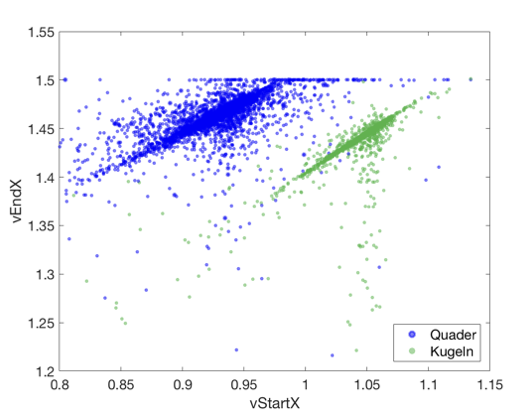
\includegraphics[width=\textwidth]{pics/Plot_Quader-Kugeln.png}
        \caption{ }
        \label{fig:PlotQuaderKugeln}
    \end{subfigure}
    \qquad
    \begin{subfigure}[b]{0.45\textwidth}
        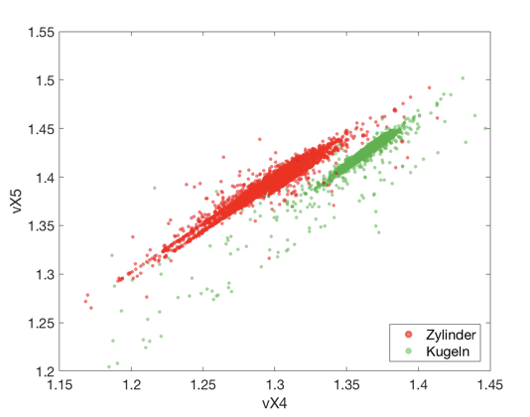
\includegraphics[width=\textwidth]{pics/Plot_Zylinder-Kugeln.png}
        \caption{ }
        \label{fig:PlotZylinderKugeln}
    \end{subfigure}
    \caption{(\ref{fig:PlotQuaderKugeln}) Plot Quader Kugeln (\ref{fig:PlotZylinderKugeln}) Plot Zylinder Kugeln}
\end{figure}


\begin{figure}
    \centering
    \begin{subfigure}[b]{0.45\textwidth}
        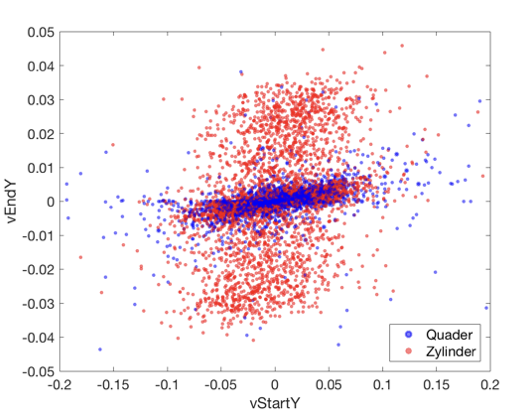
\includegraphics[width=\textwidth]{pics/Plot_Quader-Zylinder1.png}
        \caption{ }
        \label{fig:PlotQuaderZylinder1}
    \end{subfigure}
    \qquad
    \begin{subfigure}[b]{0.45\textwidth}
        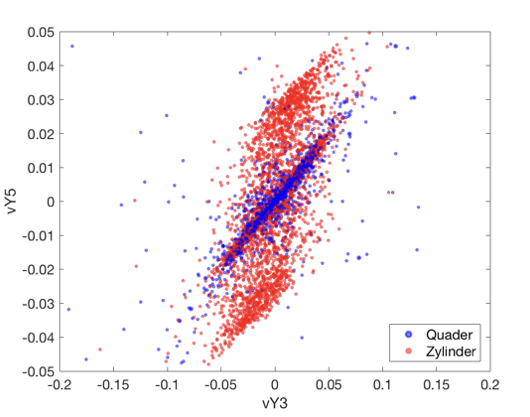
\includegraphics[width=\textwidth]{pics/Plot_Quader-Zylinder2.png}
        \caption{ }
        \label{fig:PlotQuaderZylinder2}
    \end{subfigure}
    \caption{(\ref{fig:PlotQuaderZylinder1}) Plot Quader Zylinder (\ref{fig:PlotQuaderZylinder2}) Plot Quader Zylinder}
\end{figure}


Bei der Klassifikation von Quadern und Kugeln haben wir bereits durch wenige und einfache Features eine Erkennungsrate von mehr als \textgreater0,99 erreicht. Wie man auf der Abbildung \ref{fig:PlotQuaderKugeln} sehen kann, ist es möglich mithilfe der Geschwindigkeiten am Anfang und am Ende des Fließbandes in X-Richtung eine lineare Trennung durchzuführen. Dies ist darauf zurück zu führen, dass Quader nicht direkt auf dem Fließband liegen bleiben, so nur langsam beschleunigen und damit am Anfang eine geringere Geschwindigkeit aufweisen. Die Quader und Kugel Objekte, welche die gleiche Start-Geschwindigkeit aufweisen, können mithilfe der Endgeschwindigkeit getrennt werden, da sobald die Quader Objekte auf dem Fließband liegen, sie die Geschwindigkeit des Fließbandes mit $1,5 \frac{m}{s}$ haben. Diese Geschwindigkeit wird auch nicht überschritten, wie man gut an der harten Grenze bei 1,5 in der Abbildung \ref{fig:PlotQuaderKugeln} sehen kann. 

Auch bei der Klassifikation von Zylindern und Kugeln konnten wir allein mit dem Feature VelocitiesAfterPosition eine lineare Trennung erreichen. Wie in Abbildung \ref{fig:PlotZylinderKugeln} zu sehen, hat der größte Teil der Kugelobjekte nach 60\% des Fließbandes eine höhere Geschwindigkeit als die Zylinderobjekte, da Kugeln eine höhere Eigenbewegung besitzen als Zylinder. Die Kugel- und Zylinderobjekte, welche die gleiche Geschwindigkeit nach 60\% des Fließbandes aufweisen, können mithilfe der Geschwindigkeit nach 80\% des Fließbandes getrennt werden.

Die Klassifikation von Quadern und Zylindern stellte sich als schwieriger heraus, da diese Objekte ein sehr ähnliches Verhalten haben. Dies ist verwunderlich, da physikalisch diese beiden Objekttypen sehr unterschiedlich sind. Wir gehen davon aus, dass bei der Generierung der Simulationsdaten eine zu grobe Approximation durchgeführt wurde, da ein Zylinder nur aus 8??? Seitenteilen besteht (alternativ: durch nur 32 Dreiecke approximiert wird). Wie in den Abbildungen \ref{fig:PlotQuaderZylinder1} und \ref{fig:PlotQuaderZylinder2} zu sehen, konnte mit einfachen Features nur eine Trennung von ca. 80\% erreicht werden. Mithilfe des komplexeren Features AccelerationsAfterPosition konnte jedoch eine  Erkennungsrate von mehr als \textgreater0,95 erreicht werden.

Um die Effektivität beim maschinellen Lernen von den, wie in Abschnitt \ref{Features} beschriebenen, mehr als 30  Features bewerten zu können, wurde jedes Feature einzelnen für das Training getestet. Danach wurden alle Kombinationen von zwei, drei und vier Features geprüft und verglichen. Die Ergebnisse sind...





\begin{figure}[!h]
    \centering
    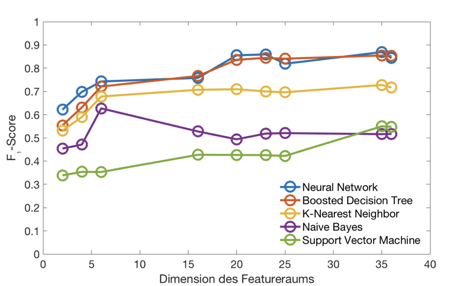
\includegraphics[width=0.7\textwidth]{pics/VergleichScores.png}
    \caption{Vergleich Scores}
    \label{fig:VergleichScores}
\end{figure}

\begin{table}[!h]
\centering
\begin{tabular}{|p{3cm}|c|c|c|c|}
  \hline & Zylinder & Quader & Leichte Kugeln & Schwere Kugeln \\
  \hline Zylinder &	  & 0,90 & \textgreater0,99 & \textgreater0,99 \\
  \hline Quader & 0,90 &   & \textgreater0,99 & \textgreater0,99 \\
  \hline Leichte Kugeln & \textgreater0,99 & \textgreater0,99 &   & \textgreater0,99 \\
  \hline Schwere Kugeln & \textgreater0,99 & \textgreater0,99 & \textgreater0,99 &   \\
  \hline

 \end{tabular}
\caption{Ergebnisse der Klassifikationen}
\label{tab:Ergebnisse}
\end{table}







\subsection{Laufzeit}

Die Klassifikation dauert pro Partikel lediglich 0,1ms. Dies lässt sich noch erhöhen, indem man statt Matlab beispielsweise C++ zur Implementierung verwendet. Somit ist eine  Echtzeitumsetzung, wie in Kapitel \ref{sec:Goal} gefordert, möglich.




\subsection{Zusammenfassung}